%%%%%%%%%%%%%%%%%%%%%%%%%%%%%%%%%%%%%%%%%%%%%%%%%%%%%%%%%%%%
%%  This Beamer template was created by Cameron Bracken.
%%  Anyone can freely use or modify it for any purpose
%%  without attribution.
%%
%%  Last Modified: January 9, 2009
%%

\documentclass[xcolor=x11names,compress]{beamer}

%% General document %%%%%%%%%%%%%%%%%%%%%%%%%%%%%%%%%%
\usepackage{graphicx}
\usepackage{tikz}
\usetikzlibrary{lindenmayersystems}
\usepackage[utf8]{inputenc}
\usepackage{verbatim}
\usepackage{fancyvrb}
\usepackage{pifont}
\usepackage{mathrsfs}
\usepackage{pmboxdraw}
\usepackage{minted}
%%%%%%%%%%%%%%%%%%%%%%%%%%%%%%%%%%%%%%%%%%%%%%%%%%%%%%
% Code snippets
\newminted{python}{fontsize=\scriptsize, 
		   framesep=3mm}

%% Beamer Layout %%%%%%%%%%%%%%%%%%%%%%%%%%%%%%%%%%
\useoutertheme[subsection=false,shadow]{miniframes}
\useinnertheme{default}
\usefonttheme{serif}
\usepackage{palatino}

\setbeamerfont{title like}{shape=\scshape}
\setbeamerfont{frametitle}{shape=\scshape}

\setbeamercolor*{lower separation line head}{bg=DeepSkyBlue4}
\setbeamercolor*{normal text}{fg=black,bg=white}
\setbeamercolor*{alerted text}{fg=red}
\setbeamercolor*{example text}{fg=black}
\setbeamercolor*{structure}{fg=black}

\setbeamercolor*{palette tertiary}{fg=black,bg=black!10}
\setbeamercolor*{palette quaternary}{fg=black,bg=black!10}

\renewcommand{\(}{\begin{columns}}
\renewcommand{\)}{\end{columns}}
\newcommand{\<}[1]{\begin{column}{#1}}
\renewcommand{\>}{\end{column}}
%%%%%%%%%%%%%%%%%%%%%%%%%%%%%%%%%%%%%%%%%%%%%%%%%%
\setbeamertemplate{caption}[numbered]       % Numbered figures
\setbeamertemplate{navigation symbols}{}    % No navigation footer
%\setbeamertemplate{footline}[page number]

\begin{document}

% Code snippets
\defverbatim[colored]\codeFactorial{
\begin{pythoncode}
def factorial(n):
    """
    Returns the factorial of n
    (int -> int)

    >>> factorial(2)
    2
    >>> factorial(3)
    6
    """
    if n:
        return n*factorial(n-1)
    else:
        return 1
\end{pythoncode}
}

\defverbatim[colored]\codeFactorialTarget{
\begin{pythoncode*}{fontsize=\huge}
@UTBP
def factorial(n):
    """
    factorial(0) == 1
    factorial(1) == 1
    factorial(2) == 2
    factorial(3) == 6
    """
\end{pythoncode*}
}

\defverbatim[colored]\codeLengthIteration{
\begin{pythoncode*}{fontsize=\large}
def length(l):
    i = 0
    for e in l:
        i += 1
    return i
\end{pythoncode*}
}

\defverbatim[colored]\codeLengthRecursion{
\begin{pythoncode*}{fontsize=\large}
def length(l):
    if l:
        return length(l[1:])+1
    else:
        return 0
\end{pythoncode*}
}

\defverbatim[colored]\codeLengthRecursionSmall{
\begin{pythoncode*}{fontsize=\scriptsize}
def length(l):
    if l: return 1+length(l[1:])
    else: return 0
\end{pythoncode*}
}





%%%%%%%%%%%%%%%%%%%%%%%%%%%%%%%%%%%%%%%%%%%%%%%%%%%%%%
%%%%%%%%%%%%%%%%%%%%%%%%%%%%%%%%%%%%%%%%%%%%%%%%%%%%%%
\begin{frame}
    \title{Programación basada en pruebas unitarias}
\author{Miguel Lechón} 
\date{28 de diciembre de 2014}
\titlepage
\end{frame}

%%%%%%%%%%%%%%%%%%%%%%%%%%%%%%%%%%%%%%%%%%%%%%%%%%%%%%
%%%%%%%%%%%%%%%%%%%%%%%%%%%%%%%%%%%%%%%%%%%%%%%%%%%%%%
%\section*{\scshape Outline}
%\begin{frame}{Outline of the presentation}
%\tableofcontents[hideallsubsections]
%\end{frame}

%%%%%%%%%%%%%%%%%%%%%%%%%%%%%%%%%%%%%%%%%%%%%%%%%%%%%%
%%%%%%%%%%%%%%%%%%%%%%%%%%%%%%%%%%%%%%%%%%%%%%%%%%%%%%
\section{\scshape Introducción}
\subsection{SIGBOVIK}
\begin{frame}{Contexto -- SigBOVIK}
    \begin{figure}[t]
        \centering
        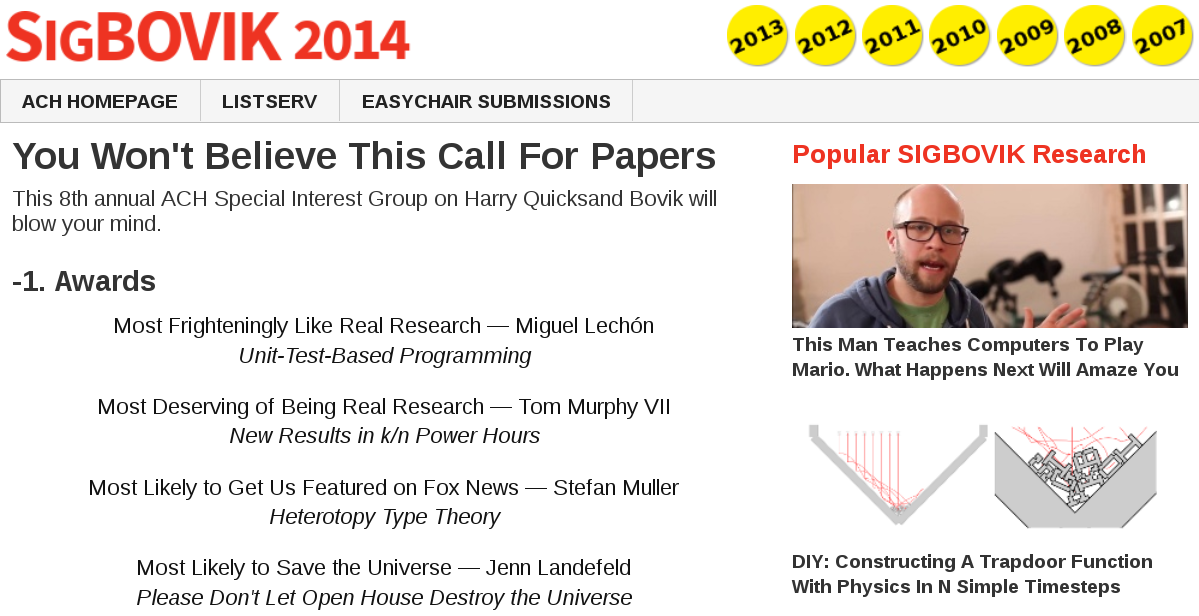
\includegraphics[width=1.0\textwidth]{images/sigbovik.png}
    \end{figure}
\end{frame}

%%%%%%%%%%%%%%%%%%%%%%%%%%%%%%%%%%%%%%%%%%%%%%%%%%%%%%
%%%%%%%%%%%%%%%%%%%%%%%%%%%%%%%%%%%%%%%%%%%%%%%%%%%%%%
\subsection{Yo}
\begin{frame}{Yo}
    \frametitle{Contexto -- Yo}
    \begin{itemize}
        \item Informático \pause
        \item Programador \textcolor{red}{sin código en producción} \pause
        \item Administrador de sistemas \textcolor{red}{mediocre} \pause
        \item Ex-estudiante de doctorado \textcolor{red}{sin doctorado} \pause
        \item Actualmente, \textcolor{blue}{ama de casa}
    \end{itemize}
\end{frame}

%%%%%%%%%%%%%%%%%%%%%%%%%%%%%%%%%%%%%%%%%%%%%%%%%%%%%%
%%%%%%%%%%%%%%%%%%%%%%%%%%%%%%%%%%%%%%%%%%%%%%%%%%%%%%
\subsection{Motivación}
\begin{frame}{Motivación}
    ¿En qué consiste programar?
    \begin{columns}
        \begin{column}{.5\linewidth}
        \begin{block}
            \codeFactorial
        \end{block}
        \end{column}
        \begin{column}{.5\linewidth}
            \begin{itemize}\itemsep25pt \pause
                \item Explicar qué se espera del código\pause
                \item Explicarlo otra vez, por si las moscas\pause
                \item Explicarlo de nuevo, esta vez para el ordenador\pause
            \end{itemize}
        \end{column}
    \end{columns}
    Uno no aprende a programar para trabajar más de la cuenta.
\end{frame}

%%%%%%%%%%%%%%%%%%%%%%%%%%%%%%%%%%%%%%%%%%%%%%%%%%%%%%
%%%%%%%%%%%%%%%%%%%%%%%%%%%%%%%%%%%%%%%%%%%%%%%%%%%%%%
\subsection{Objetivo}
\begin{frame}{Objetivo}
    \pause
    \codeFactorialTarget
\end{frame}


%%%%%%%%%%%%%%%%%%%%%%%%%%%%%%%%%%%%%%%%%%%%%%%%%%%%%%
%%%%%%%%%%%%%%%%%%%%%%%%%%%%%%%%%%%%%%%%%%%%%%%%%%%%%%
\subsection{Pero\ldots ¿cómo?}
\begin{frame}{Pero\ldots ¿cómo?}
    Premisas:
    \pause
    \begin{itemize}
        \item Toda función se puede escribir de forma recursiva \pause
        \item Toda función recursiva puede representarse mediante un árbol \pause
        \item Los árboles se pueden enumerar en order creciente de complejidad \pause
    \end{itemize}
    Conclusión:

    \textbf{$\rightarrow$ Podemos enumerar todas las funciones de forma ordenada} \pause

    (y comprobar, una a una, si satisfacen nuestras pruebas unitarias)
\end{frame}

%%%%%%%%%%%%%%%%%%%%%%%%%%%%%%%%%%%%%%%%%%%%%%%%%%%%%%
%%%%%%%%%%%%%%%%%%%%%%%%%%%%%%%%%%%%%%%%%%%%%%%%%%%%%%

\section{\scshape Discusión sesuda}

\subsection{Toda función se puede escribir de forma recursiva}
\begin{frame}{Funciones: todas recursivas}
    \textcolor{red}{Advertencia:} Este es un ejercicio académico \pause extremadamente complejo\pause. Gritad si os perdéis. \pause
    \begin{columns}
        \begin{column}{.30\linewidth}
        \begin{block}
            \codeLengthIteration
        \end{block}
        \end{column}
        \begin{column}{.65\linewidth}
        \begin{block}
            \codeLengthRecursion
        \end{block}
        \end{column}
    \end{columns} \pause
    La versión recursiva es claramente superior.
\end{frame}

%%%%%%%%%%%%%%%%%%%%%%%%%%%%%%%%%%%%%%%%%%%%%%%%%%%%%%
%%%%%%%%%%%%%%%%%%%%%%%%%%%%%%%%%%%%%%%%%%%%%%%%%%%%%%

\subsection{Expresiones como árboles}
\begin{frame}[fragile]
    \frametitle{Expresiones como árboles}
    $$\frac{-b\pm\sqrt{b^2-4ac}}{2a}$$

\begin{Verbatim}[commandchars=\\\{\},codes={\catcode`$=3\catcode`_=8}]
        \textbf{/}
        ├── \textbf{+/-}
        │   ├── \textbf{neg}
        │   │   └── b
        │   └── \textbf{sqrt}
        │       └── \textbf{-}
        │           ├── \textbf{^}
        │           │   ├── b
        │           │   └── 2
        │           └── \textbf{*}
        │               ├── 4
        └── \textbf{*}           └── \textbf{*}
            ├── 2           ├── a
            └── a           └── c
\end{Verbatim}
\end{frame}



\subsection{Toda función recursiva puede representarse mediante un árbol}
\begin{frame}[fragile]
    \frametitle{Funciones recursivas: todas árboles}
    \codeLengthRecursionSmall
\begin{Verbatim}[commandchars=\\\{\},codes={\catcode`$=3\catcode`_=8}]
\textbf{python}                \textbf{pseudo-scheme}
def                   define                    
  length              ├── length                
                      └── lambda                
(l):                      ├── l                 
    if                    └── if                
      l:                      ├── l             
        return 1+             ├── succ          
            length(           │   └── length    
                l[1:]         │       └── cdr   
            )                 │           └── l 
    else: return 0            └── 0             
\end{Verbatim}

\end{frame}

\subsection{Brain-body-niche}
\begin{frame}{Brain-body-niche}

\begin{itemize}
    \item \emph{No need to dissociate brain from body or body from environment}
    \item \emph{Who needs internal representations when you're part of the system you're trying to represent?}
    \item \emph{No computation}
\end{itemize}
\end{frame}

\subsection{Multifractal fractality}
\begin{frame}{Multifractal fractality}
\begin{itemize}
    \item \emph{Power-laws imply complexity. Exponents, exponents!}
    \item \emph{Forget about computation. Let's talk about energy flow.}
    \item \emph{No computation}
\end{itemize}

\end{frame}

\section{\scshape Criticism}
\subsection{Criticism}
\begin{frame}{Criticism}
    Approach taken by three of the articles
    \begin{itemize}
        \item \emph{Detect 1/f noise in time series of human performance}
            \begin{itemize}
                \item Competing models?
                \item Frailty of the measure
            \end{itemize}
        \item \emph{The presence of 1/f noise implies an interaction dominant system}
            \begin{itemize}
                \item Other systems can also generate 1/f noise
                \item Generation of 1/f noise in complex systems depends on specific circumstances
            \end{itemize}
        \item \emph{Cognition is interaction-dominant and traditional approaches should be abandoned}
            \begin{itemize}
                \item The complex systems approach should explain something that traditional approaches cannot explain.
                \item Model instead of ``solving'' by dropping terms like self-organized criticality
            \end{itemize}
    \end{itemize}
\end{frame}

\subsection{Piles of rice and salt}
\begin{frame}{Piles of rice and salt}
\end{frame}

\subsection{Does this apply to us?}
\begin{frame}{Does this apply to us?}
    I don't think much of the discussion applies to us (the original Frontiers article should not have confronted Wagenmakers and Friston and we \emph{do} talk about components as well as their interactions), however\ldots
    \begin{itemize}
        \item Do we make our best effort to disprove criticality? Competing hypotheses.
        \item Do we try to model something other than 1/f?
    \end{itemize}
\end{frame}

%%%%%%%%%%%%%%%%%%%%%%%%%%%%%%%%%%%%%%%%%%%%%%%%%%%%%%
%%%%%%%%%%%%%%%%%%%%%%%%%%%%%%%%%%%%%%%%%%%%%%%%%%%%%%

\section{\scshape Doubts}
\subsection{Doubts}
\begin{frame}{Doubts}
I'm no statistical physicist and I should not take on blind faith some of 
    \begin{itemize}
        \item Power-laws and fractals
        \item Power-laws and complexity
    \end{itemize}
\end{frame}

\end{document}
